\documentclass[11pt,a4paper]{article}

\usepackage{Act}


\begin{document}
\input{\detokenize{/home/fenarius/Travail/Cours/cpge-info/latex/Macros.tex}}
\newcommand{\SPATH}{/home/fenarius/Travail/Cours/cpge-info/docs/mp2i/files/}

\ModeExercice

\Colles{S21/S22/S23}{Structures de données}

\setboolean{corrige}{true}

\setcounter{Exercise}{0}

\begin{Exercise}[title = {Nombre d'arêtes}]
    \Question{Rappeler la définition d'un arbre binaire.}
    \tcor{Voir cours}
    \Question{Soit $a$ un arbre binaire à $n$ noeuds ($n \geqslant 1$), montrer que $a$ possède $n-1$ arêtes.}
    \tcor{Preuve par récurrence forte sur la taille de l'arbre ($k$ noeuds dans le sous arbre gauche et $n-k-1$ noeuds dans le sous arbre droit), il faut distignuer le cas où l'un des sous arbre est vide.  }
    \Question{On rappelle l'implémentation des arbres en OCaml utilisée en cours :
    \inputpartOCaml{\SPATH/C12/abi.ml}{}{}{1}{3}
    En utilisant cette implémentation, écrire une fonction {\tt nb\_aretes} de signature {\tt ab -> int} et qui renvoie le nombre d'arêtes d'un arbre binaire
    }
    \tcor{En utilisant le résultat de la question précédente, il suffit de calculer la taille de l'arbre, on traite le cas de l'arbre vide avec un {\tt failwith}:
    \inputpartOCaml{ab.ml}{}{}{103}{111}
    }
\end{Exercise}


\begin{Exercise}[title = {Parcours d'arbre binaires}] 
\Question{Donner l'ordre des noeuds lors des parcours prefixe, infixe et postfixe de l'arbre suivant : \\
\pstree[arrows=->,treesep=0.8cm,levelsep=1cm]{\TCircle{\tt 29}}
        {\pstree{\TCircle{\tt 24}}
        {\pstree{\TCircle{\tt 14}}
        { \Tn{} 
        \pstree{\TCircle{\tt 16}}
        { \Tn{} 
        \TCircle{\tt 20} 
        }}\TCircle{\tt 28} 
        }\pstree{\TCircle{\tt 31}}
        { \Tn{} 
        \TCircle{\tt 30} }}}
        \tcor{\begin{itemize}
            \item préfixe : {\tt [ 29; 24; 14; 16; 20; 28; 31; 30 ]}
            \item infixe : {\tt [ 14; 16; 20; 24; 28; 29; 31; 30 ]}
            \item postfixe : {\tt [ 20; 16; 14; 28; 24; 30; 31; 29 ]}
        \end{itemize}
        }
\Question{On cherche à présent à reconstruire un arbre en connaissant un ou plusieurs de ses parcours. Montrer sur un exemple que deux arbres ayant les mêmes parcours prefixe et postfixe peuvent être différents.}
\tcor{On peut prendre un peigne}
\Question{Montrer (en le construisant) qu'un seul arbre a pour préfixe [ 0; 1; 2; 3; 4; 5; 6; 7 ] et pour parcours infixe
[ 1; 2; 0; 5; 4; 6; 3; 7 ]}
\tcor{
    \begin{center}
        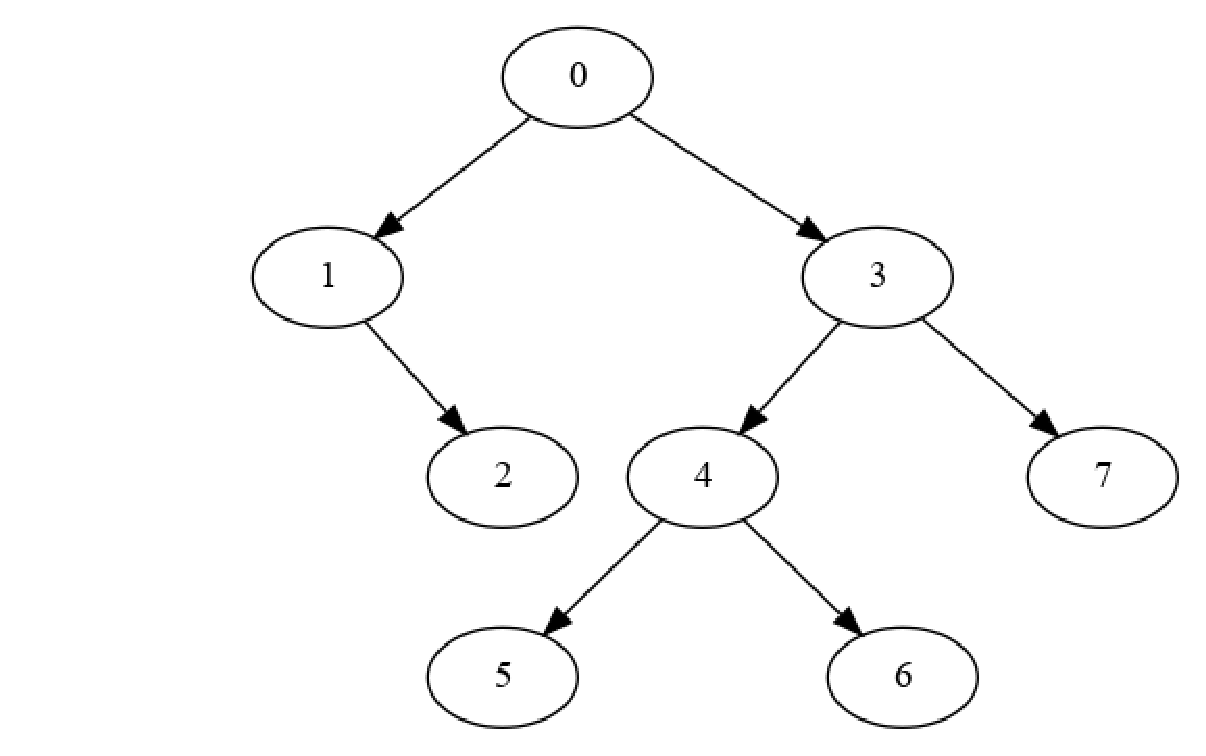
\includegraphics[width=200px]{sol.eps}
    \end{center}
}
\Question{Comment savoir si deux listes de valeurs correspondent aux parcours prefixe et infixe d'un arbre binaire ?}
\tcor{On note $p = [p_0, \dots p_{n-1}]$ et $i = [i_0, \dots i_{n-1}]$ les listes représentant les parcours prefixe et infixe. Comme ce sont les parcours du même arbre, $i$ est une permutation de $p$. On extrait deux sous listes $i_g$ et $i_d$ de $i$, $i_g$ sont les éléments situés à gauche de $p_0$ et $i_d$ ceux situés à droite. On extrait de même deux sous listes de $p$, $p_g$ contient les $|i_g|$ éléments situés après $p_0$ et $p_d$ le reste de la liste. La liste $p_g$ doit être une permutation de $i_g$ et $p_d$ doit être une permutation de $i_d$. Et cette propriété doit rester vraie en reproduisant ce processus récursivement sur les deux listes extraites.}
\Question{Ecrire une fonction qui prend en argument deux listes (le parcours prefixe et le parcours infixe) et qui renvoie l'arbre binaire correspondant. On supposera que les étiquettes de l'arbre sont des entiers tous différents.
\aide \; On pourra commencer par écrire :
\begin{itemize}
    \item Une fonction {\tt separe\_valeur} de signature {\tt int -> int list -> int list * int list} qui prend en argument un entier, une liste contenant cet entier et renvoie un couple de liste : les élément situés avant (resp après) cette valeur
    \item Une fonction {\tt separe\_nb} de signature {\tt int -> int list -> int list * int list} qui prend en argument un entier {\tt n} et une liste et renvoie un couple de listes : les {\tt n} éléments situés après le premier puis le reste de la liste.
\end{itemize}
}
\end{Exercise}


\begin{Exercise}[title = {Expression bien parenthésée}]\\
    On considère dans cet exercice un parenthésage avec les couples $()$, $\{\}$ et  $[]$. On dira qu'une expression est bien parenthésée si chaque symbole ouvrant correspond à un symbole fermant et si l'expression contenue à l'intérieur est elle-même bien parenthésée.
    \Question{Les expressions suivantes sont-elles bien parenthésée ?
    \begin{itemize}
     \item[\textbullet] $3+[5-4\div(3+2)]\}+10$
     \item[\textbullet] $\{(3+2)\times 5$ 
     \item[\textbullet] $5)-4\times2($ 
     \item[\textbullet] $[(3+2)\times(5-3)]$
    \end{itemize}
    \Question{Rappeler les fonctions de l'interface d'une pile.}
    \Question{Ecrire une fonction {\tt bien\_parenthesee} de signature {\tt str -> bool} qui renvoie {\tt true} lorsque la chaine de caractère donnée en argument est une expression bien parenthésée \\
    \aide \; on utilisera le module {\tt Stack} de OCaml afin de disposer d'une structure de pile \textit{mutable}. On rappelle ci-dessous les fonctions principales de ce module :
    \begin{itemize}
        \item \mintinline{ocaml}{Stack.create} de signature {\tt () -> 'a t} qui crée une pile vide d'éléments de type {\tt 'a}. Par exemple \mintinline{ocaml}{let mapile = Stack.create ()}
        \item \mintinline{ocaml}{Stack.push} de signature {\tt 'a 'a t -> ()} qui empile un élément. Par exemple \mintinline{ocaml}{Stack.push 5 mapile} empile l'entier 5 sur {\tt mapile} (le type option 'a est alors le type {\tt int}).
        \item \mintinline{ocaml}{Stack.pop} de signature {\tt 'a t -> 'a} qui renvoie l'élément situé au sommet de la pile en le dépilant.
    \end{itemize}
    }
    }
\end{Exercise}

\begin{Exercise}
    \Question{Rappeler la définition du type abstrait \textit{file} et donner les fonctions de son interface.}
    \Question{On rappelle que lorsque la file a une capacité bornée $N$, on peut l'implémenter en utilisant un tableau {\tt tab} de taille $N$ qu'on traite de façon circulaire. On maintient alors à jour :
    \begin{itemize}
        \item une variable {\tt size}  contenant le nombre d'élément de la file
        \item une variable {\tt next} contenant l'indice du prochain élément à défiler
    \end{itemize}
    Expliciter les opérations enfiler et défiler en terme de modification sur {\tt tab}, {\tt size} et {\tt next}.
    }
    \Question{Dans le cas où $N=3$, décrire le contenu de {\tt tab} et des variables {\tt size} et {\tt next} lorsqu'on effectue les opérations suivante : enfiler 2, enfiler 3, défiler, enfiler 4, défiler, enfiler 7, enfiler 8.}
    \Question{Donner une implémentation en OCaml en utilisant le type suivant :
    \inputpartOCaml{ringbuffer.ml}{}{}{1}{6}
    }
\end{Exercise}

\begin{Exercise}[title = {Comptine enfantine}]\\
    Certaines comptines enfantines ont pour objectif de désigner une personne \og{} au hasard \fg{}, un exemple bien connu est \og{} \textit{Am, stram, gram, pic et pic et colégram} \fg{}. On suppose que $N$ enfants numérotés de 0 à $N-1$ sont assis en cercle et que l'un d'entre eux (le numéro $k$) récite une comptine contenant $S$ syllabes. A la première syllable il désigne son suivant immédiat dans le cercle puis il avance d'un enfant à chaque syllable jusqu'à la fin de la comptine. L'enfant désigné à la fin de la comptine doit quitter le cercle et le processus recommence à partir de son suivant immédiat jusqu'à ce qu'un seul enfant reste.
    \Question{Donner une illustration de ce processus avec $N=5$ et $S=7$, en supposant que l'enfant $0$ commence.}
    \Question{Implémenter en OCaml, un programme exécutant ce processus et donnant le numéro de l'enfant restant. On pourra utiliser le module {\tt Queue} de OCaml. Dont on rappelle ci-dessous les fonctions principales :
    \begin{itemize}
        \item \mintinline{ocaml}{Queue.create}  qui crée une file vide d'éléments de type {\tt 'a}. 
        \item \mintinline{ocaml}{Queue.add}  qui enfile un élément. 
        \item \mintinline{ocaml}{Queue.take} qui défile
    \end{itemize}}
\end{Exercise}

\begin{Exercise}[title = {Tester si un arbre est un {\sc abr}}]

\Question{Rappeler la définition d'un arbre binaire de recherche}
\Question{Proposer deux méthodes de complexité linéaire permettant de vérifier qu'un arbre est bien un {\sc abr}.}
\Question{Donner l'implémentation de l'une au moins des méthodes.}

\end{Exercise}


\begin{Exercise}[title = {Recherche dans un {\sc abr}}]
    \Question{Rappeler la définition d'un arbre binaire de recherche}
    \Question{On suppose maintenant qu'on a inséré dans un {\sc abr} initialement vide tous les entiers compris en 0 et 999. On effectue la recherche de l'entier 666 dans cet arbre. Parmi les séquences de valeurs suivantes, lesquelles peuvent être la séquence de noeuds parcourus jusqu'à  atteindre 666 ? :
    \begin{itemize}
        \item 487, 503, 911, 954, 499, 651, 672, 668, 666
        \item 951, 812, 803, 798, 751, 670, 589, 652, 653, 666
        \item 985, 112, 251, 306, 444, 503, 574, 602, 605, 681, 666
        \item 844, 511, 845, 603, 702, 651, 699, 660, 670, 665, 666
        \item 303, 404, 541, 752, 749, 742, 592, 603, 666
    \end{itemize}}
    \Question{Proposer un algorithme qui prend en entrée une séquence d'entiers $u_0, \dots u_{n}$ avec $u_n$ la valeur cherchée et vérifie que cette séquence peut effectivement constituer la suite de noeuds visités lors de la recherche réussie d'un nombre dans un tel {\sc abr}. L'algorithme doit avoir une complexité temporelle en $O(n)$.}
    \Question{En fournir une implémentation en OCaml, en supposant que la séquence est donnée sous la forme d'un tableau d'entiers de OCaml. La signature de votre fonction sera donc {\tt int array -> bool}}
    \Question{Soit $t$ un tableau représentant la suite de valeurs obtenue lors de la recherche réussie d'un élément dans un {\sc abr}, proposer un algorithme \textit{de complexité linéaire} permettant de trier ce tableau. En donner l'implémentation en OCaml.}
\end{Exercise}

\begin{Exercise}[title = {Collision dans une table de hachage}]\\
        Pour une chaine de caractères $s = c_0\dots c_{n-1}$, on considère la fonction de hachage :
        $$ h(s) = \sum_{i=0}^{n-1} 31^i \times c_i$$
        \Question{Calculer le hash de la chaine {\tt "AB"}.}
        \Question{Montrer qu'il existe deux chaines de caractères de longueur 2, formées de lettres minuscules (code 97 à 177) ou majuscules (code 65 à 90) et produisant la même valeur pour $h$.}
        \Question{En déduire une façon de construire un nombre arbitraire de chaînes de caractères de longueurs quelconques ayant la même valeur pour la fonction $h$. \label{qu}}
        \Question{Pour implémenter cette fonction en langage C, on propose une fonction de signature \mintinline{c}{int hash(char *s)}. Qu'en pensez-vous ?}
        \Question{Proposer une implémentation \textit{efficace} pour cette fonction en langage C.}
        \Question{Déterminer, grâce à la question \ref{qu}, deux chaines de 8 caractères produisant une collision et le vérifier.}
\end{Exercise}
    

\end{document}